\chapter{Appendix Example and Some Guidance}
\label{appx:methods}

\doublespacing
\noindent Note that appendices still use double-spacing for text. Additionally, to comply with the formatting guidance that appendices should not use table / figure numbering and should instead reference only the appendix itself, you can use the * to remove prevent number. For example \texttt{\textbackslash caption*\{DHS displacement procedure visualization\}}.

You can include multiple appendix files, but in this example, I have included only one.

\begin{itemize}
    \item \textbf{Step 1:} A random angle is drawn
    \item \textbf{Step 2:} Random distance (between 0 km and 2 km in urban areas, between 0 km and 5 km in rural, with 1\% of rural clusters displaced between 0 and 10 km)
    \item \textbf{Step 3:} If displaced location falls outside of admin boundary (the district level in Malawi), the steps 1 and 2 are repeated.
\end{itemize}

\begin{figure}[H]
  \centering
    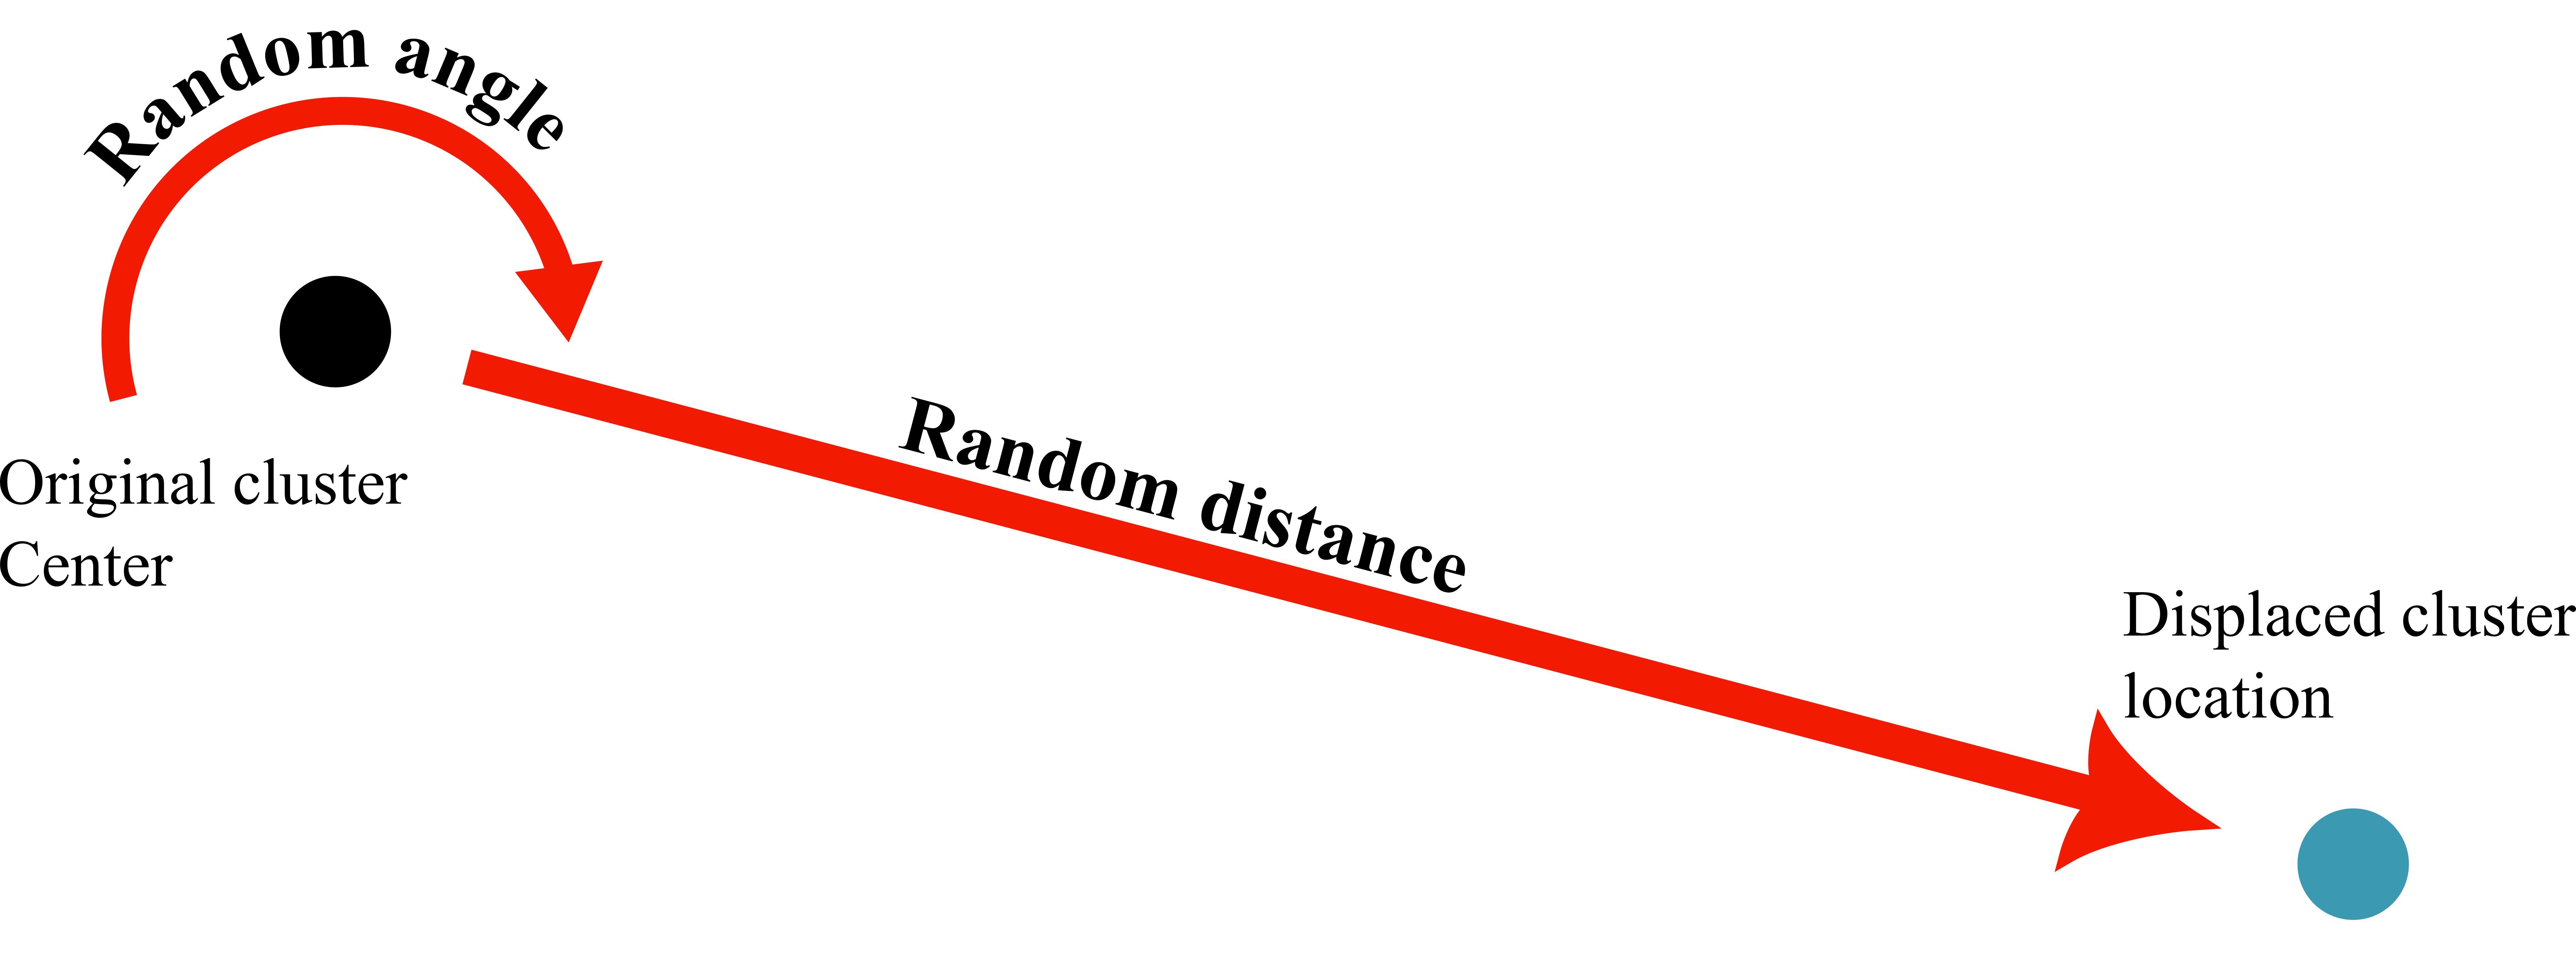
\includegraphics[width=6in]{images/displacement.png}
  % 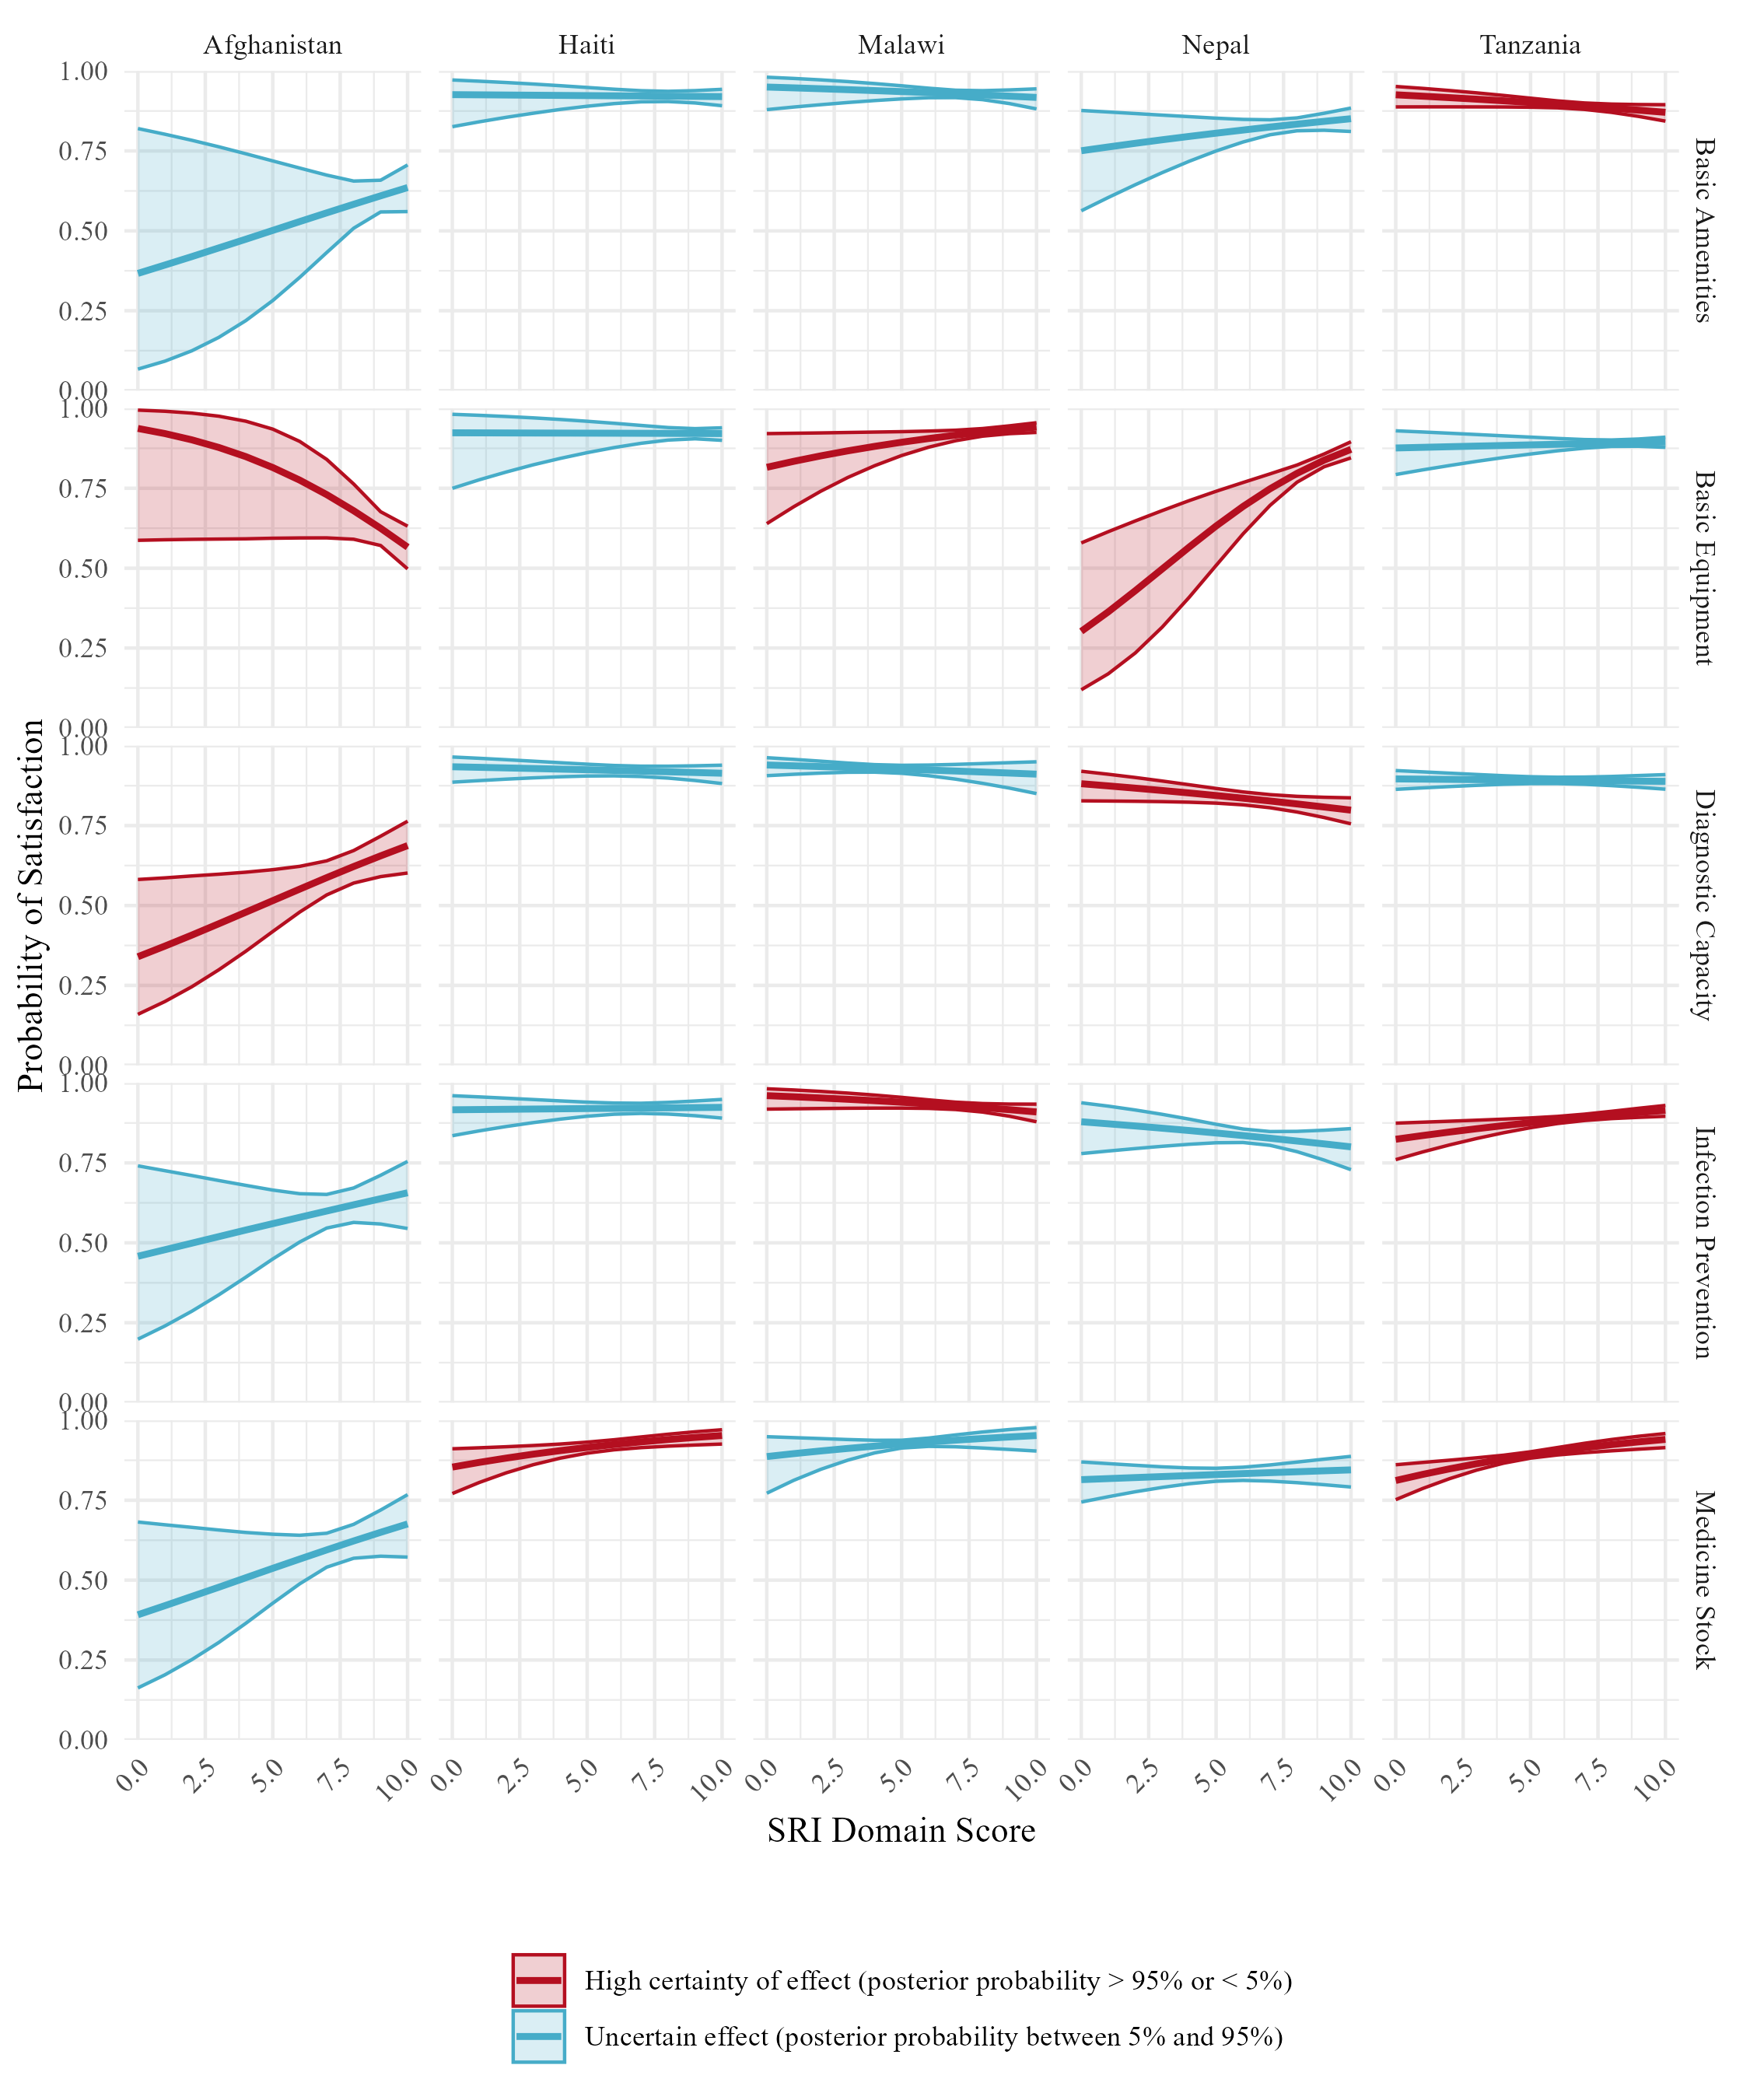
\includegraphics[width=7.5in, height=9in]{images/an_marginalEffects.png}
  \caption*{DHS displacement procedure visualization}
  \label{fig-displacement}
\end{figure}

Proin venenatis mattis convallis. Morbi cursus pulvinar lorem, vel fringilla nibh bibendum sit amet. Phasellus ut lacus bibendum mi facilisis sodales. Pellentesque ultricies risus vitae viverra hendrerit. Fusce lobortis, dolor vel fringilla lobortis, tellus nibh ultricies lectus, quis placerat quam est a elit. Phasellus at quam finibus neque condimentum euismod sit amet nec est. Sed nec mollis nibh, a dapibus justo. Sed turpis lectus, lacinia quis sapien non, suscipit venenatis diam. Nunc facilisis ut arcu eu gravida. Sed felis sem, semper in sodales a, sodales a lacus. Sed lacinia nec nunc a ornare. Donec id nulla metus. Praesent viverra egestas justo, quis elementum dui posuere ac. Sed a condimentum velit, sit amet egestas eros. Nam iaculis, odio vel pharetra placerat, diam justo molestie sapien, sit amet fringilla massa magna id erat. 

% \[
% f_j(s)=
% \begin{cases}
% \dfrac{1}{2\pi r_j d(s,\tilde{s}_j)}, & d(s,\tilde{s}_j)\le r_j,\\[6pt]
% 0, & \text{otherwise},
% \end{cases}
% \]
    \begin{equation}
    \label{eq:pdf}
f_j(x_{0},y_{0}) = 
\begin{dcases}
\frac{1}{2\pi r_j\sqrt{x_{0}^{2}+y_{0}^{2}}}, & \text{if } 0 < \sqrt{x_{0}^2 + y_{0}^2} \leq r_j \\
0, & \text{otherwise.}
\end{dcases}
\end{equation}

\noindent where $x_0$ and $y_0$ denote projected coordinate offsets from the released cluster location $\tilde{s}_j$, and the singularity at $\sqrt{x_0^2+y_0^2}=0$ can be ignored in practice by excluding the zero-distance point from integral calculations.

Nam maximus et dolor a luctus. Integer bibendum, ante eu pellentesque pharetra, nibh ex condimentum ex, vitae eleifend dui lectus nec magna. Nulla sagittis faucibus eros ut tincidunt. Aenean commodo accumsan est, eget elementum nibh malesuada eget. Praesent tempor quam non lacus malesuada, ac sollicitudin enim sodales. Proin at enim elementum magna vulputate semper. 


\begin{figure}[H]
  \centering
    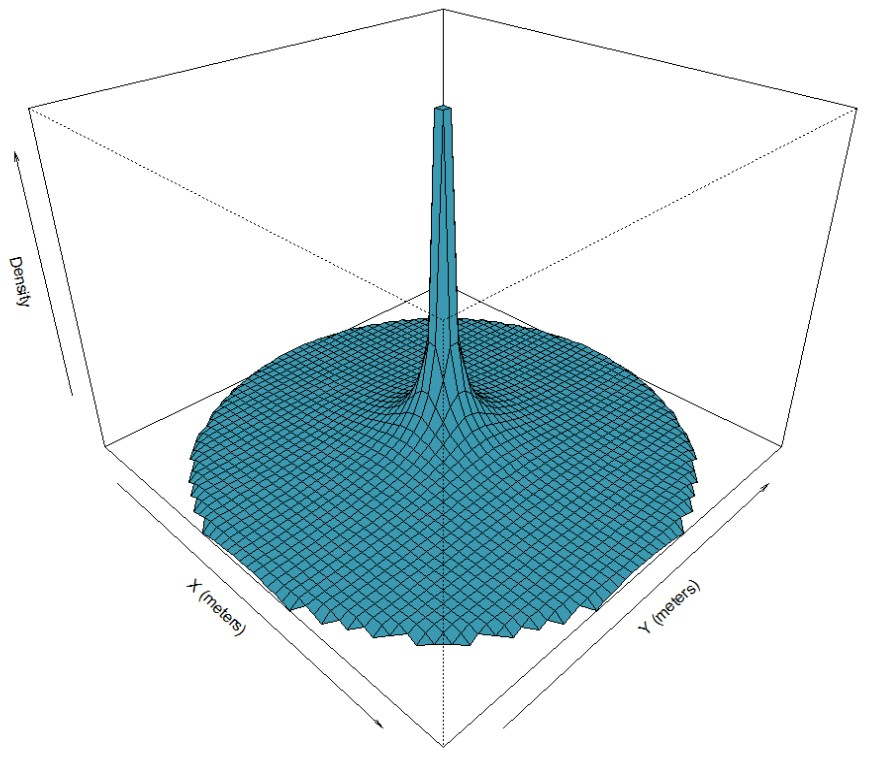
\includegraphics[height=4in]{images/DensityPlot.jpg}
  % 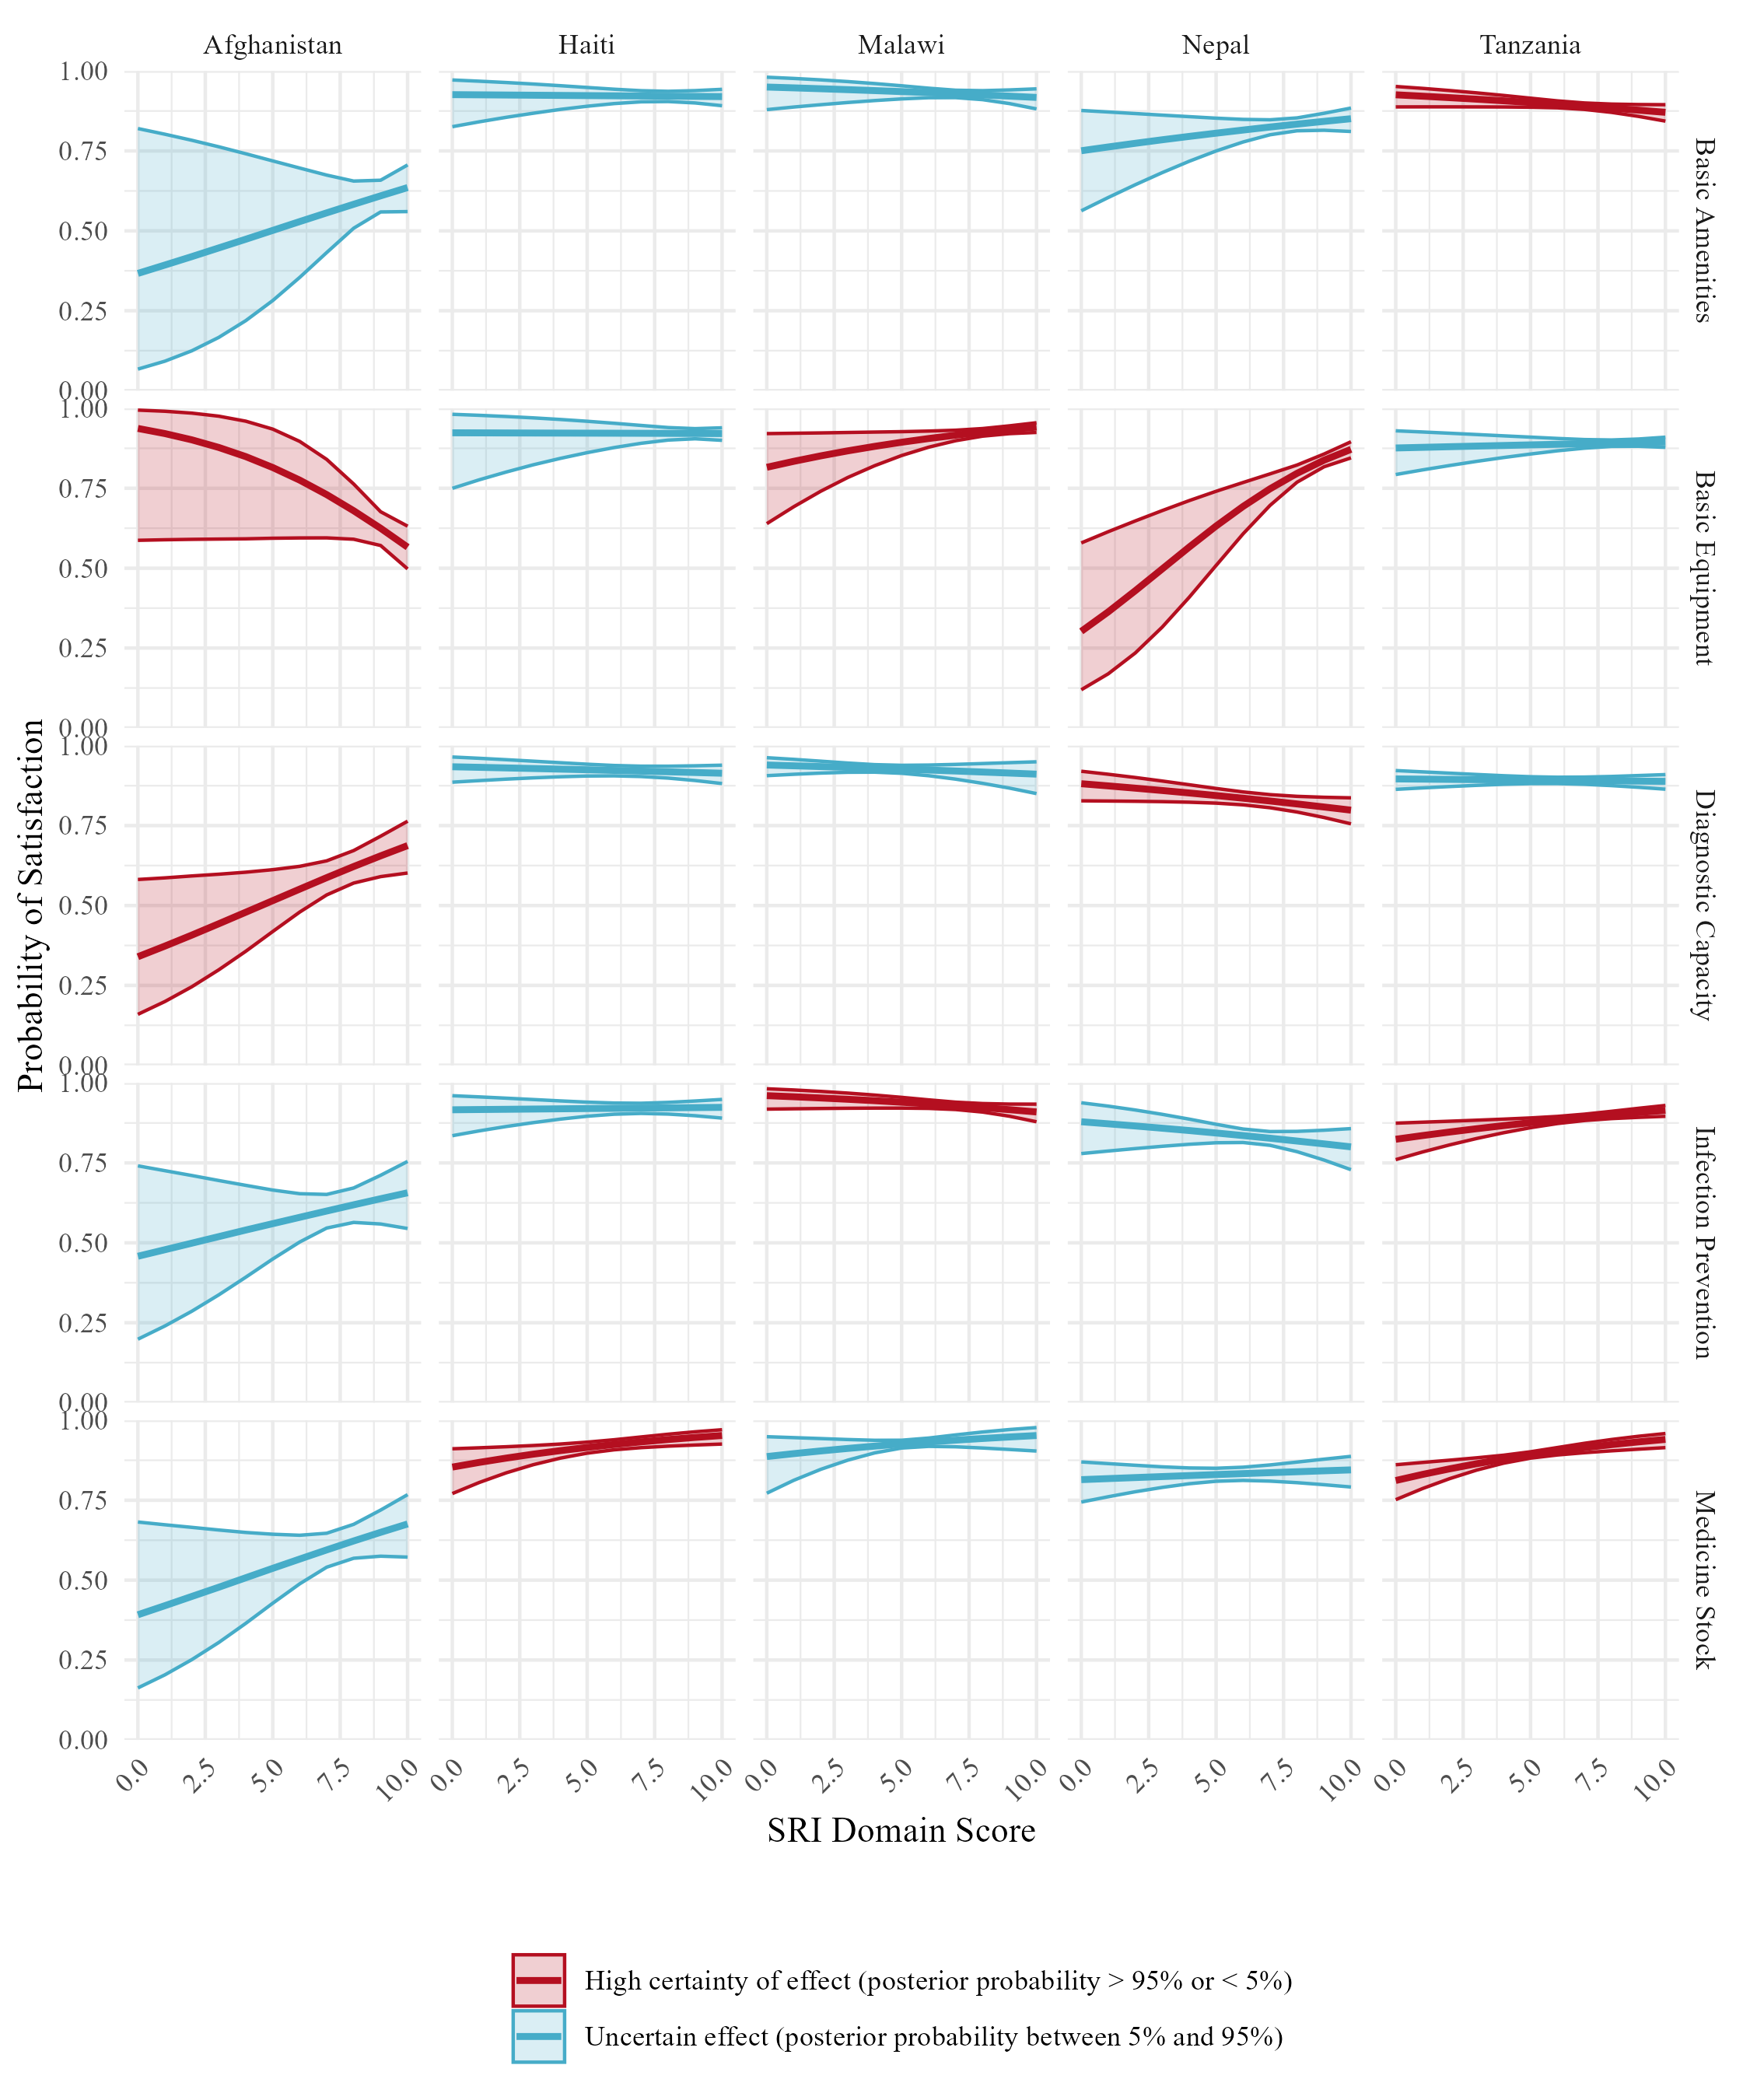
\includegraphics[width=7.5in, height=9in]{images/an_marginalEffects.png}
  \caption*{Visualization of the surface created by the equation above}
  \label{fig-pdf_plot}
\end{figure}

 Nunc viverra rhoncus nulla, pretium interdum erat scelerisque quis. Cras ornare, libero et bibendum semper, quam elit accumsan tortor, sed efficitur libero ipsum non velit. Donec at justo suscipit, viverra arcu vestibulum, volutpat enim. Integer sed dapibus nunc. Nulla interdum nisl ligula, quis facilisis justo vestibulum et. Cras consequat egestas fringilla. Vestibulum nec commodo arcu, sit amet condimentum neque. Maecenas sed magna posuere, dignissim quam sit amet, euismod enim. Vivamus semper viverra turpis, eget viverra felis. Integer gravida molestie ex. Nam maximus et dolor a luctus. Integer bibendum, ante eu pellentesque pharetra, nibh ex condimentum ex, vitae eleifend dui lectus nec magna.



\chapter{Sensitivity tests using half-Cauchy priors for the random intercept standard deviation}
\label{appx:half-cauchy}

\begin{table}[H]
\centering
\begin{threeparttable}

\singlespacing    
\caption*{Sensitivity analysis: Bayesian multilevel logistic regression models for antenatal care utilization, Malawi, using a half-Cauchy prior for the cluster-level random intercept standard deviation. Posterior median odds ratios (OR), 95\% credible intervals, and posterior probability of direction (PD).}
\label{tbl:app_anc_models_halfcauchy_mw}
{\fontsize{11pt}{13.2pt}\selectfont
\begin{tabular}{l ll ll}
\hline
\hline
 & \multicolumn{2}{c}{4+ ANC visits} & \multicolumn{2}{c}{ANC initiation (1st trimester)} \\
 & OR & PD$^{\dagger}$ & OR & PD$^{\dagger}$ \\
 & 95\% CrI &  & 95\% CrI &  \\
\hline

\textbf{Health service environment (cluster-level)} & & & & \\
\hspace{2pt} Essential medicines readiness (0--10) & 1.05 & 99.6\% & 1.05 & 99.0\% \\
 & (1.01 -- 1.08) & & (1.01 -- 1.10) & \\
\hspace{2pt} Service availability (days/month) & 1.00 & 74.1\% & 1.00 & 80.0\% \\
 & (0.99 -- 1.01) & & (0.99 -- 1.01) & \\
\hspace{2pt} Pr(nearest facility charges fees) (per 10pp)$^{\S}$ & 1.00 & 57.0\% & 0.98 & 100.0\% \\
 & (0.99 -- 1.01) & & (0.96 -- 0.99) & \\
\hspace{2pt} Distance to nearest facility (km) & 0.98 & 98.2\% & 0.99 & 84.1\% \\
 & (0.96 -- 1.00) & & (0.96 -- 1.01) & \\

\textbf{Individual and household characteristics} & & & & \\
\hspace{2pt} Rural residence & 0.95 & 75.4\% & 1.16 & 94.8\% \\
 & (0.81 -- 1.11) & & (0.97 -- 1.41) & \\
\hspace{2pt} Household wealth (quintile) & 1.03 & 97.9\% & 1.06 & 99.9\% \\
 & (1.00 -- 1.07) & & (1.02 -- 1.10) & \\
\hspace{2pt} Maternal age at index birth (years) & 1.03 & 100.0\% & 1.02 & 99.7\% \\
 & (1.02 -- 1.04) & & (1.00 -- 1.03) & \\
\hspace{2pt} Respondent education (years) & 1.03 & 100.0\% & 1.01 & 97.1\% \\
 & (1.01 -- 1.04) & & (1.00 -- 1.03) & \\
\hspace{2pt} Parity (birth order) & 0.94 & 100.0\% & 0.95 & 99.5\% \\
 & (0.91 -- 0.97) & & (0.92 -- 0.99) & \\

\hline
\textit{Random intercept SD (cluster)} & 0.40 & & 0.53 & \\
 & (0.34 -- 0.45) & & (0.47 -- 0.60) & \\
Observations & 13,448 & & 13,448 & \\
Clusters (DHSID) & 850 & & 850 & \\
\hline

% \multicolumn{5}{p{16cm}}{\footnotesize
% ORs are posterior medians from Bayesian multilevel logistic regression models with a cluster-level random intercept (DHSID). Cluster-level health service environment measures were constructed using a probabilistic linkage procedure accounting for DHS geographic displacement. Sensitivity models used a half-Cauchy prior for the cluster-level random intercept standard deviation (see Appendix \ref{appx:half-cauchy}). Credible intervals are equal-tailed (95\%). 
% $^{\dagger}$ The posterior probability of direction (PD) is the posterior probability that the estimated effect is strictly positive or strictly negative (whichever is larger), reflecting the strength of evidence for the direction of the association. 
% $^{\S}$ Fee exposure is scaled such that a one-unit increase corresponds to a 10 percentage-point increase in the probability that the nearest facility charges fees.}

\end{tabular}

\begin{tablenotes}[flushleft]
\fontsize{9pt}{10.5pt}\selectfont
\setlength{\itemsep}{0pt}
\setlength{\parsep}{0pt}
\setlength{\leftskip}{0pt}
\item ORs are posterior medians from Bayesian multilevel logistic regression models with a cluster-level random intercept (DHSID). Cluster-level health service environment measures were constructed using a probabilistic linkage procedure accounting for DHS geographic displacement. Sensitivity models used a half-Cauchy prior for the cluster-level random intercept standard deviation (see Appendix \ref{appx:half-cauchy}). Credible intervals are equal-tailed (95\%). 
$^{\dagger}$ The posterior probability of direction (PD) is the posterior probability that the estimated effect is strictly positive or strictly negative (whichever is larger), reflecting the strength of evidence for the direction of the association. 
$^{\S}$ Fee exposure is scaled such that a one-unit increase corresponds to a 10 percentage-point increase in the probability that the nearest facility charges fees.
\end{tablenotes}

}
\end{threeparttable}
\end{table}





\restoregeometry